\documentclass{article}
\usepackage[utf8]{inputenc}
\usepackage{graphicx}
\usepackage{hyperref}

\title{Lab 03- ARP Poisoning and DHCP Security}
\author{Matthew Belanger}
\date{\today}

\begin{document}

\maketitle

\newpage

% SECTION 1

% TASK 1

\section{Task 1: ARP Poisoning Attack}
\label{sec:task1}

\section*{Tasks}

\subsection{\textbf{Environment Setup}: Create a simple network with two virtual machines (VM1 and VM2) connected
through a virtual switch or host-only network. Ensure both VMs can ping each other, confirming
network connectivity.}

See Figure \ref{fig:connected}

\begin{figure}[h]
    \centering
    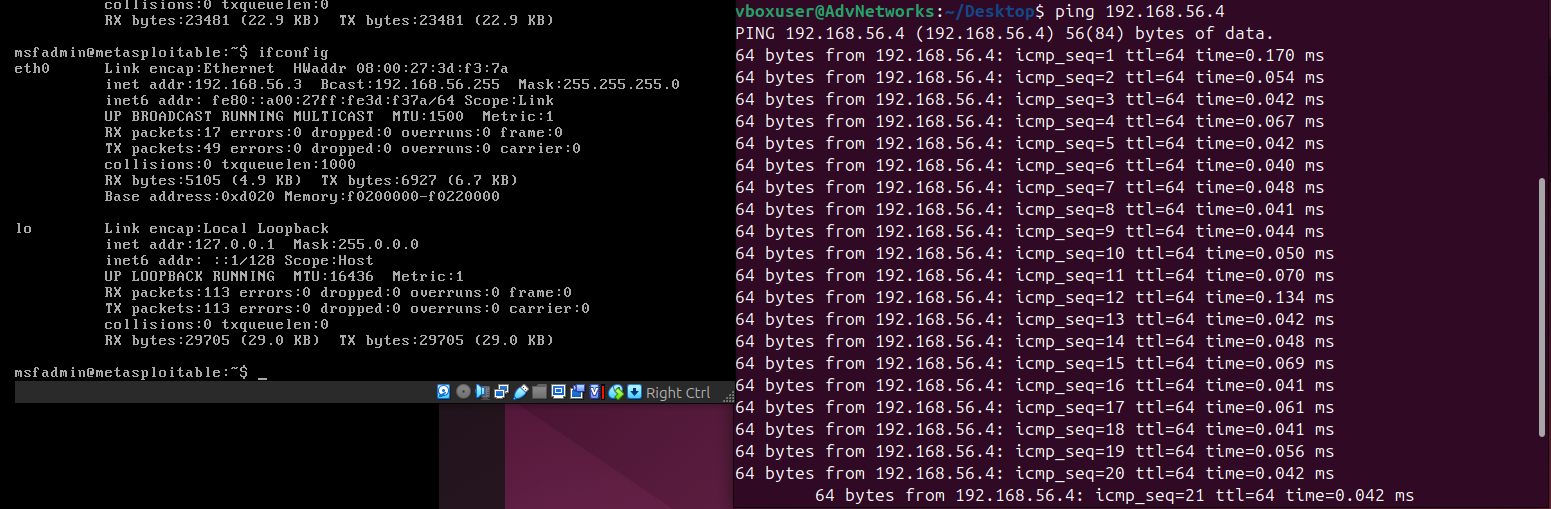
\includegraphics[width=0.8\textwidth]{task1/screenshot/connected.png}
    \caption{VMs Connected}
    \label{fig:connected}
\end{figure}


\subsection{\textbf{ARP Security Testing}: Write a script using Scapy to perform ARP security testing (pentesting), follow the STRIDE methodology we applied in the class to test and verify the identified vulnerabilities.}

See code \href{https://github.com/MattBelanger321/COMP8670/tree/master/lab3/task1}{Repo}

\subsection{\textbf{Mitigation and Report}: Discuss and implement basic mitigation strategies against ARP poisoning,
such as static ARP entries or using ARP spoofing detection tools.}

\subsubsection{Spoofing}  
To detect and block unauthorized ARP messages, implement ARP inspection or dynamic ARP inspection mechanisms.

\subsubsection{Tampering}  
Mitigate the risks of ARP cache poisoning by using techniques such as ARP cache timeouts or static ARP entries. Additionally, deploy network-based intrusion detection systems (IDS) to monitor and alert on suspicious ARP activity.

\subsubsection{Repudiation}  
To prevent replay attacks, include sequence numbers or timestamps in ARP messages. Deploy network monitoring tools to detect and identify unusual ARP message patterns.

\subsubsection{Information Disclosure}  
To protect ARP traffic from eavesdropping, use encryption protocols like IPsec. Additionally, use network segmentation to restrict the visibility of ARP traffic to authorized devices only.

\subsubsection{Denial of Service}  
Implement rate limiting for ARP messages to avoid overwhelming network devices with excessive traffic. Also, deploy intrusion prevention systems (IPS) to detect and block ARP flood attacks.

\subsubsection{Elevation of Privilege}  
Use secure communication protocols like HTTPS or SSH to safeguard sensitive data from interception. In addition, apply network segmentation and access control measures to minimize the impact of compromised devices.

\label{subsubsec:arp-mit}

\section*{Report Requirements}

\subsection*{Network configurations and ARP tables before and after the attack.}

\subsubsection*{Before}

See Figure \ref{fig:before}

\begin{figure}[h]
    \centering
    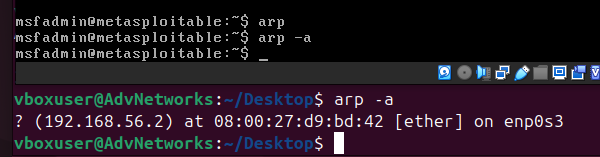
\includegraphics[width=0.8\textwidth]{task1/screenshot/before.png}
    \caption{VMs Connected}
    \label{fig:before}
\end{figure}

\subsubsection*{After}

See Figure \ref{fig:after}

I am pretending to be the DHCP server here. You can see the ARP table has two IPs with the same MAC. 

\begin{figure}[h]
    \centering
    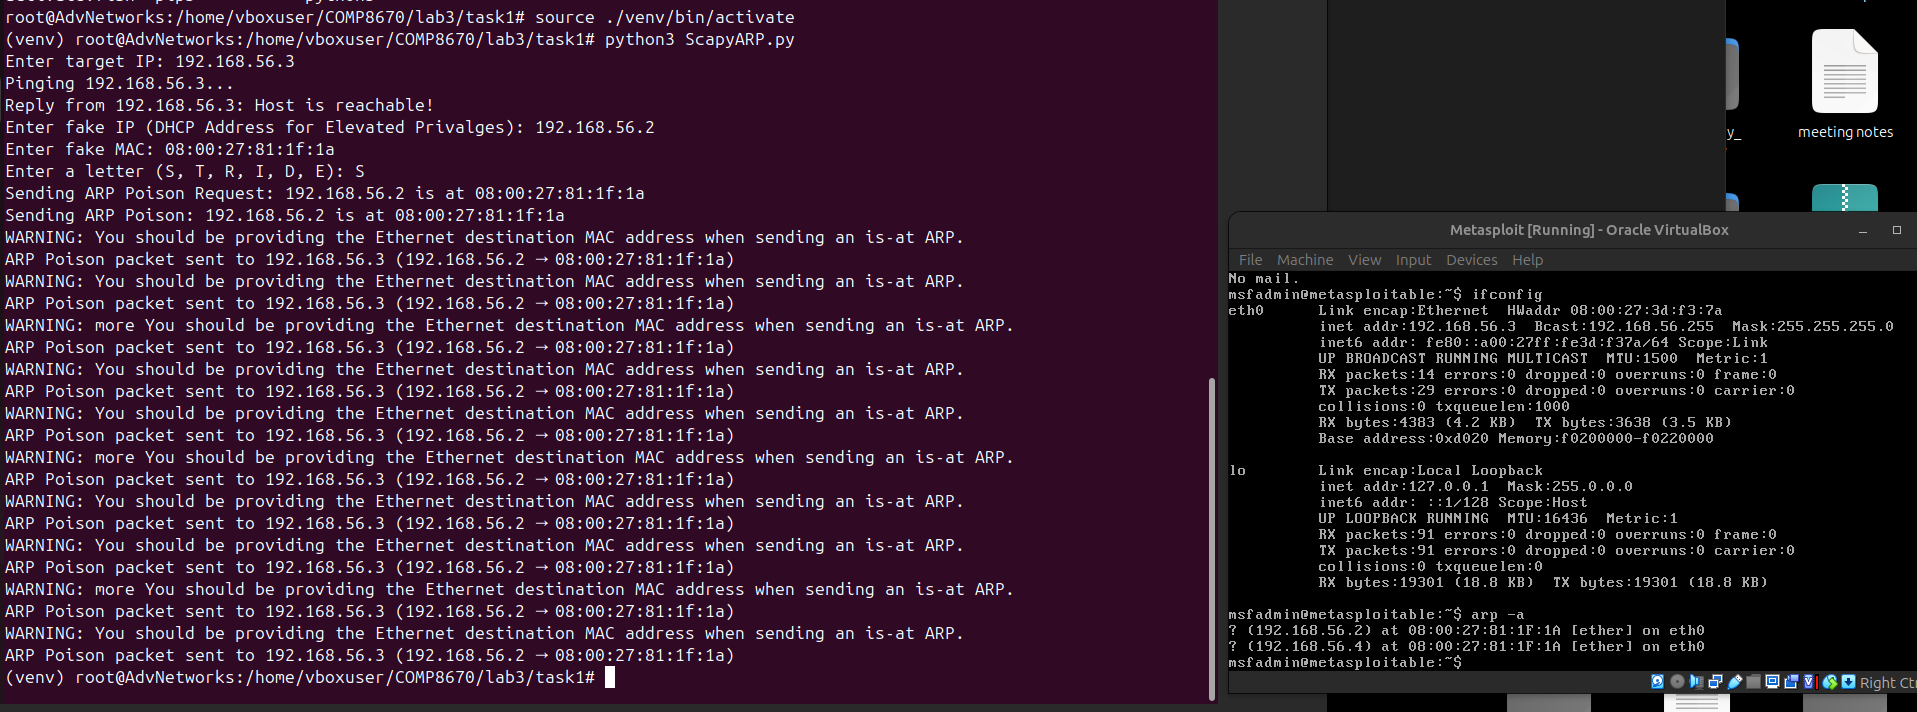
\includegraphics[width=0.8\textwidth]{task1/screenshot/poison.png}
    \caption{Poisoning Screenshot}
    \label{fig:after}
\end{figure}

\subsection*{Scapy scripts used.}

See code \href{https://github.com/MattBelanger321/COMP8670/tree/master/lab3/task1}{Repo}

\subsection*{Screenshots demonstrating the success of the attack, including Wireshark captures.}

In figure \ref{fig:wireshark-proof} I pretend to be the DHCP server at 192.168.56.2 (actual IP 192.168.56.4). On the victim machine I ping the DHCP server but the packets are recieved on hackers machine.

\begin{figure}[h]
    \centering
    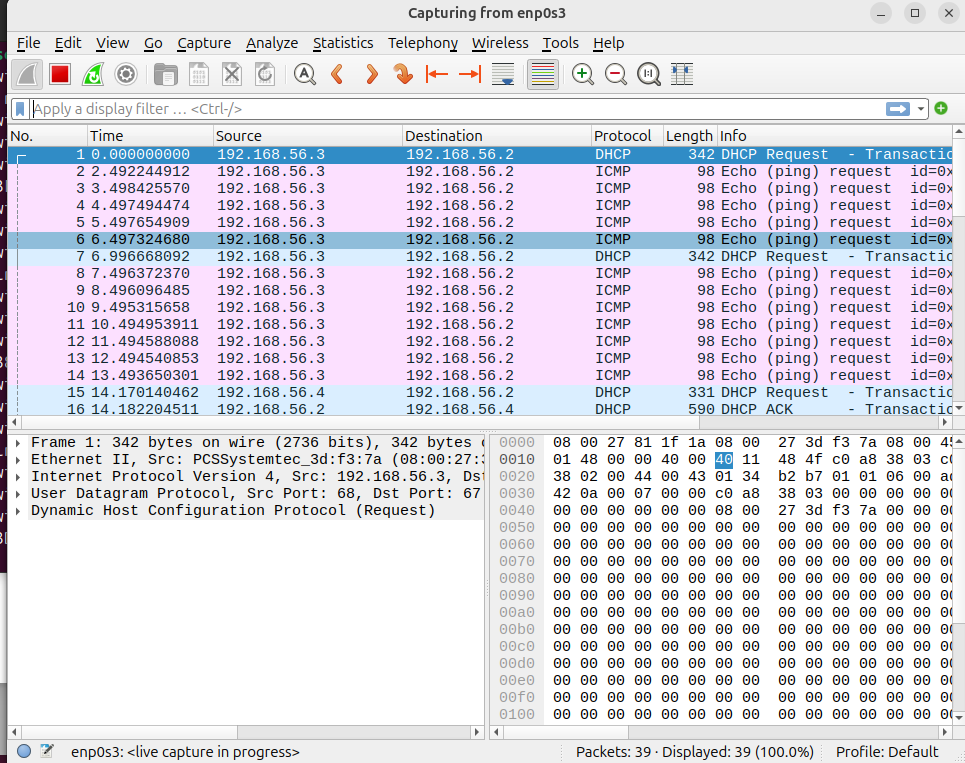
\includegraphics[width=0.8\textwidth]{task1/screenshot/wireshark_spoof_proof.png}
    \caption{Wireshark Spoof}
    \label{fig:wireshark-proof}
\end{figure}

\subsection*{Discussion on mitigation strategies.}

See section \ref{subsubsec:arp-mit}

\newpage

% TASK 2

\section{Task 2: Security Analysis of The DHCP}

\subsection{Start Wireshark open the enclosed pcap trace file and list all the DHCP packets in the trace. Use
screenshots to support your answer.}

See Figure \ref{fig:pcap_dhcp}

\begin{figure}[h]
    \centering
    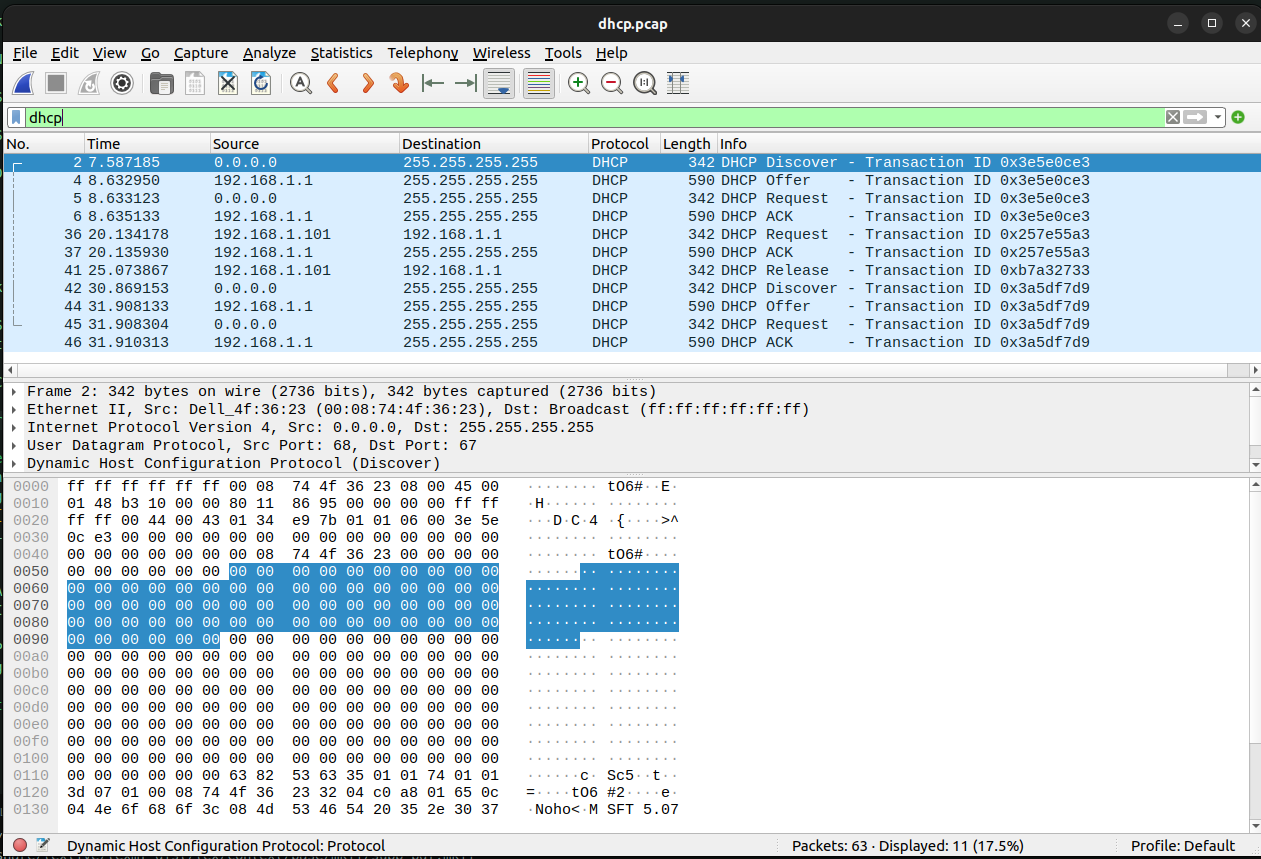
\includegraphics[width=0.8\textwidth]{task2/dhcp_wireshark.png}
    \caption{DHCP Packet List}
    \label{fig:pcap_dhcp}
\end{figure}

\subsection{Create a Finite State Machine model for the DHCP process.}
 
See Figure \ref{fig:dhcp_fsm}. The FSM is largely based on DORA.

\begin{figure}[h]
    \centering
    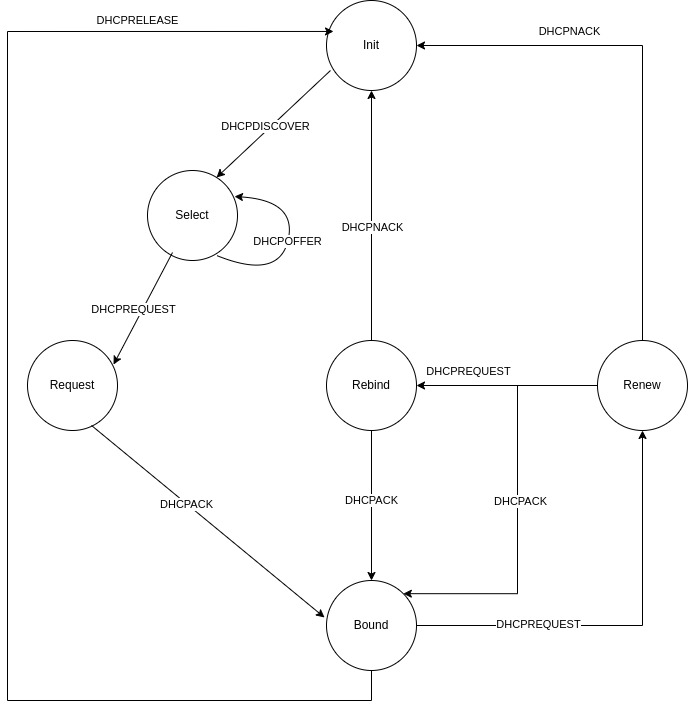
\includegraphics[width=0.8\textwidth]{task2/DHCP_FSM.jpg}
    \caption{DHCP Finite State Machine}
    \label{fig:dhcp_fsm}
\end{figure}

\subsection{Apply the STRIDE methodology to the FSM model of DHCP to identify potential security threats.
For each STRIDE element, identify possible vulnerabilities in the DHCP process.}

\subsubsection{Spoofing}  
In the DORA process, a malicious entity could spoof DHCP messages to impersonate a legitimate DHCP server or client. This could occur at the \textbf{DHCP Discover} and \textbf{DHCP Offer} stages, where an attacker sends a fraudulent DHCP Offer pretending to be the server. This leads clients to configure their network settings with malicious or incorrect information, potentially redirecting traffic or enabling man-in-the-middle attacks.

\subsubsection{Tampering}  
Tampering could occur if an attacker intercepts and alters DHCP messages during the DORA process. The most vulnerable stages are \textbf{DHCP Offer} and \textbf{DHCP Acknowledgment}, where an attacker could modify these messages to provide a malicious IP address, subnet mask, DNS server, or other settings. This could cause traffic redirection, service disruption, or exposure of sensitive information.

\subsubsection{Repudiation}  
Repudiation could occur during the \textbf{DHCP Request} or \textbf{DHCP Acknowledgment} stages if there is no logging or mechanism to ensure the legitimacy of the messages. If a client or server denies receiving a message, such as a DHCP Offer or Acknowledgment, it becomes difficult to track malicious actions or resolve network issues related to IP assignment, causing confusion in troubleshooting or network management.

\subsubsection{Information Disclosure}  
In DHCP, information disclosure could occur at any stage of the DORA process, especially during the unencrypted transmission of DHCP messages. A malicious actor could intercept DHCP Discover, Offer, or Acknowledgment messages to gain sensitive information about the network configuration, such as DNS server addresses, default gateways, or other parameters that could be used for further attacks.

\subsubsection{Denial of Service}  
A Denial of Service (DoS) attack could happen at the \textbf{DHCP Discover} stage, where an attacker floods the network with DHCP Discover messages (also known as DHCP starvation). This could exhaust the pool of available IP addresses on the server, causing legitimate clients to be unable to obtain an IP address and resulting in network downtime.

\subsubsection{Elevation of Privilege}  
An attacker could exploit vulnerabilities in the DHCP process to elevate privileges by impersonating a legitimate device during the \textbf{DHCP Discover} or \textbf{DHCP Request} stages. By tricking the DHCP server into assigning an IP address and network configuration to a compromised device, an attacker could gain unauthorized access to restricted networks or sensitive systems, thus escalating privileges within the network.

\subsection{Propose mitigation strategies for each identified vulnerability. This could involve protocol enhancements, configuration changes, or additional security mechanisms.}

\subsubsection{Spoofing}  
To mitigate spoofing in the DORA process, implement DHCP authentication mechanisms such as DHCP Secure (DHCP-S) or use cryptographic techniques like digital signatures to verify the legitimacy of DHCP messages. Additionally, network devices can be configured to only accept DHCP offers from trusted servers. Using static IP assignments for critical devices and employing port security in switches to restrict DHCP responses can also reduce the risk of spoofing.

\subsubsection{Tampering}  
Tampering can be mitigated by encrypting DHCP messages to prevent unauthorized modifications. Protocols like IPsec or DHCP over TLS can be employed to ensure integrity and confidentiality of messages between DHCP clients and servers. Additionally, using secure communication channels for DHCP transactions and implementing message authentication codes (MACs) can help detect and prevent tampered messages.

\subsubsection{Repudiation}  
To prevent repudiation, ensure proper logging and auditing of DHCP transactions at every stage of the DORA process. Logs should include detailed information about requests, offers, and acknowledgments, including timestamps and unique identifiers. Implementing a secure logging system and using non-repudiation techniques, such as digital signatures, can also help ensure that no entity can deny having participated in the DHCP process.

\subsubsection{Information Disclosure}  
To mitigate information disclosure, DHCP messages should be encrypted using IPsec or another secure transport protocol. This prevents attackers from eavesdropping on network configuration details such as DNS servers and gateways. Network segmentation and using VLANs to restrict the scope of DHCP traffic to only authorized devices can also limit exposure to sensitive information.

\subsubsection{Denial of Service}  
To prevent DoS attacks, implement rate-limiting on DHCP requests to prevent excessive message flooding. Use DHCP snooping to ensure that only legitimate DHCP servers are allowed to issue offers to clients. Additionally, configuring the DHCP server to handle requests efficiently and implementing redundant DHCP servers can help prevent service disruption. Intrusion Prevention Systems (IPS) can also be used to detect and block DoS attempts targeting the DHCP process.

\subsubsection{Elevation of Privilege}  
To mitigate elevation of privilege, secure communication between DHCP clients and servers with encryption and strong authentication mechanisms. Implement network access control to restrict access to DHCP servers and sensitive network resources. Furthermore, the use of port security on switches and dynamic IP address filtering can prevent unauthorized devices from connecting to the network and obtaining IP addresses from the DHCP server.


\end{document}
